%%%% Preamble
\documentclass[paper=a4, fontsize=11pt]{scrartcl}

%%AGREG0
\usepackage{float}
%\usepackage{geometry}
%\geometry{verbose,tmargin=2cm,bmargin=2cm,lmargin=2cm,rmargin=2cm,headheight=2cm,headsep=2cm}
%\geometry{verbose,tmargin=2cm,bmargin=2cm,lmargin=2cm,rmargin=2cm,headheight=2cm,headsep=2cm}

\usepackage[T1]{fontenc}
\usepackage{fourier}
\usepackage[utf8]{inputenc}
\usepackage[english]{babel}					% English language/hyphenation

\usepackage[protrusion=true,expansion=true]{microtype}	
\usepackage{amsmath,amsfonts,amsthm} % Math packages
\usepackage[pdftex]{graphicx}	
\usepackage{url}
\usepackage{import}

\usepackage[margin=2cm]{geometry}
\geometry{verbose,tmargin=2cm,bmargin=2cm,lmargin=2cm,rmargin=2cm,headheight=2cm,headsep=2cm}
% %%% Custom sectioning
\usepackage{sectsty}
\allsectionsfont{\normalfont \scshape}


%%% Custom headers/footers (fancyhdr package)
\usepackage{fancyhdr}
\pagestyle{fancyplain}
\fancyhead{}											% No page header
\fancyfoot[L]{}											% Empty 
\fancyfoot[C]{}											% Empty
\fancyfoot[R]{\thepage}									% Pagenumbering
\renewcommand{\headrulewidth}{0pt}			% Remove header underlines
\renewcommand{\footrulewidth}{0pt}				% Remove footer underlines
\setlength{\headheight}{13.6pt}


%%% Equation and float numbering
\numberwithin{equation}{section}		% Equationnumbering: section.eq#
\numberwithin{figure}{section}			% Figurenumbering: section.fig#
\numberwithin{table}{section}				% Tablenumbering: section.tab#


%%% Maketitle metadata
\newcommand{\horrule}[1]{\rule{\linewidth}{#1}} 	% Horizontal rule

%AGREGO PARA EJ 1
\usepackage{graphicx}
\usepackage{color} 
\usepackage[dvipsnames]{xcolor}
\colorlet{purple}{purple}

%/////////////////////////////////// AGREGO PARA EL EJ 2

    \usepackage{geometry} % Required to change the page size to A4
    \geometry{a4paper} % Set the page size to be A4 as opposed to the default US Letter

    \usepackage{mathtools, nccmath}
    
    \usepackage{tikz}
    \usetikzlibrary{matrix,calc}

    %isolated term
%#1 - Optional. Space between node and grouping line. Default=0
%#2 - node
%#3 - filling color
\newcommand{\implicantsol}[3][0]{
    \draw[rounded corners=3pt, fill=#3, opacity=0.3] ($(#2.north west)+(135:#1)$) rectangle ($(#2.south east)+(-45:#1)$);
    }


%internal group
%#1 - Optional. Space between node and grouping line. Default=0
%#2 - top left node
%#3 - bottom right node
%#4 - filling color
\newcommand{\implicant}[4][0]{
    \draw[rounded corners=3pt, fill=#4, opacity=0.3] ($(#2.north west)+(135:#1)$) rectangle ($(#3.south east)+(-45:#1)$);
    }

%group lateral borders
%#1 - Optional. Space between node and grouping line. Default=0
%#2 - top left node
%#3 - bottom right node
%#4 - filling color
\newcommand{\implicantcostats}[4][0]{
    \draw[rounded corners=3pt, fill=#4, opacity=0.3] ($(rf.east |- #2.north)+(90:#1)$)-| ($(#2.east)+(0:#1)$) |- ($(rf.east |- #3.south)+(-90:#1)$);
    \draw[rounded corners=3pt, fill=#4, opacity=0.3] ($(cf.west |- #2.north)+(90:#1)$) -| ($(#3.west)+(180:#1)$) |- ($(cf.west |- #3.south)+(-90:#1)$);
}

%group top-bottom borders
%#1 - Optional. Space between node and grouping line. Default=0
%#2 - top left node
%#3 - bottom right node
%#4 - filling color
\newcommand{\implicantdaltbaix}[4][0]{
    \draw[rounded corners=3pt, fill=#4, opacity=0.3] ($(cf.south -| #2.west)+(180:#1)$) |- ($(#2.south)+(-90:#1)$) -| ($(cf.south -| #3.east)+(0:#1)$);
    \draw[rounded corners=3pt, fill=#4, opacity=0.3] ($(rf.north -| #2.west)+(180:#1)$) |- ($(#3.north)+(90:#1)$) -| ($(rf.north -| #3.east)+(0:#1)$);
}

%group corners
%#1 - Optional. Space between node and grouping line. Default=0
%#2 - filling color
\newcommand{\implicantcantons}[2][0]{
    \draw[rounded corners=3pt, opacity=.3] ($(rf.east |- 0.south)+(-90:#1)$) -| ($(0.east |- cf.south)+(0:#1)$);
    \draw[rounded corners=3pt, opacity=.3] ($(rf.east |- 8.north)+(90:#1)$) -| ($(8.east |- rf.north)+(0:#1)$);
    \draw[rounded corners=3pt, opacity=.3] ($(cf.west |- 2.south)+(-90:#1)$) -| ($(2.west |- cf.south)+(180:#1)$);
    \draw[rounded corners=3pt, opacity=.3] ($(cf.west |- 10.north)+(90:#1)$) -| ($(10.west |- rf.north)+(180:#1)$);
    \fill[rounded corners=3pt, fill=#2, opacity=.3] ($(rf.east |- 0.south)+(-90:#1)$) -|  ($(0.east |- cf.south)+(0:#1)$) [sharp corners] ($(rf.east |- 0.south)+(-90:#1)$) |-  ($(0.east |- cf.south)+(0:#1)$) ;
    \fill[rounded corners=3pt, fill=#2, opacity=.3] ($(rf.east |- 8.north)+(90:#1)$) -| ($(8.east |- rf.north)+(0:#1)$) [sharp corners] ($(rf.east |- 8.north)+(90:#1)$) |- ($(8.east |- rf.north)+(0:#1)$) ;
    \fill[rounded corners=3pt, fill=#2, opacity=.3] ($(cf.west |- 2.south)+(-90:#1)$) -| ($(2.west |- cf.south)+(180:#1)$) [sharp corners]($(cf.west |- 2.south)+(-90:#1)$) |- ($(2.west |- cf.south)+(180:#1)$) ;
    \fill[rounded corners=3pt, fill=#2, opacity=.3] ($(cf.west |- 10.north)+(90:#1)$) -| ($(10.west |- rf.north)+(180:#1)$) [sharp corners] ($(cf.west |- 10.north)+(90:#1)$) |- ($(10.west |- rf.north)+(180:#1)$) ;
}

%Empty Karnaugh map 4x4
\newenvironment{Karnaugh}%
{
\begin{tikzpicture}[baseline=(current bounding box.north),scale=0.8]
\draw (0,0) grid (4,4);
\draw (0,4) -- node [pos=0.7,above right,anchor=south west] {y2 y1} node [pos=0.75,below left,anchor=north east] {w y3} ++(135:1);
%
\matrix (mapa) [matrix of nodes,
        column sep={0.8cm,between origins},
        row sep={0.8cm,between origins},
        every node/.style={minimum size=0.3mm},
        anchor=8.center,
        ampersand replacement=\&] at (0.5,0.5)
{
                       \& |(c00)| 00         \& |(c01)| 01         \& |(c11)| 11         \& |(c10)| 10         \& |(cf)| \phantom{00} \\
|(r00)| 00             \& |(0)|  \phantom{0} \& |(1)|  \phantom{0} \& |(3)|  \phantom{0} \& |(2)|  \phantom{0} \&                     \\
|(r01)| 01             \& |(4)|  \phantom{0} \& |(5)|  \phantom{0} \& |(7)|  \phantom{0} \& |(6)|  \phantom{0} \&                     \\
|(r11)| 11             \& |(12)| \phantom{0} \& |(13)| \phantom{0} \& |(15)| \phantom{0} \& |(14)| \phantom{0} \&                     \\
|(r10)| 10             \& |(8)|  \phantom{0} \& |(9)|  \phantom{0} \& |(11)| \phantom{0} \& |(10)| \phantom{0} \&                     \\
|(rf) | \phantom{00}   \&                    \&                    \&                    \&                    \&                     \\
};
}%
{
\end{tikzpicture}
}

%Empty Karnaugh map 2x4
\newenvironment{Karnaughvuit}%
{
\begin{tikzpicture}[baseline=(current bounding box.north),scale=0.8]
\draw (0,0) grid (4,2);
\draw (0,2) -- node [pos=0.7,above right,anchor=south west] {y2 y1} node [pos=0.7,below left,anchor=north east] {y3} ++(135:1);
%
\matrix (mapa) [matrix of nodes,
        column sep={0.8cm,between origins},
        row sep={0.8cm,between origins},
        every node/.style={minimum size=0.3mm},
        anchor=4.center,
        ampersand replacement=\&] at (0.5,0.5)
{
                      \& |(c00)| 00         \& |(c01)| 01         \& |(c11)| 11         \& |(c10)| 10         \& |(cf)| \phantom{00} \\
|(r00)| 0             \& |(0)|  \phantom{0} \& |(1)|  \phantom{0} \& |(3)|  \phantom{0} \& |(2)|  \phantom{0} \&                     \\
|(r01)| 1             \& |(4)|  \phantom{0} \& |(5)|  \phantom{0} \& |(7)|  \phantom{0} \& |(6)|  \phantom{0} \&                     \\
|(rf) | \phantom{00}  \&                    \&                    \&                    \&                    \&                     \\
};
}%
{
\end{tikzpicture}
}

%Empty Karnaugh map 2x2
\newenvironment{Karnaughquatre}%
{
\begin{tikzpicture}[baseline=(current bounding box.north),scale=0.8]
\draw (0,0) grid (2,2);
\draw (0,2) -- node [pos=0.7,above right,anchor=south west] {b} node [pos=0.7,below left,anchor=north east] {a} ++(135:1);
%
\matrix (mapa) [matrix of nodes,
        column sep={0.8cm,between origins},
        row sep={0.8cm,between origins},
        every node/.style={minimum size=0.3mm},
        anchor=2.center,
        ampersand replacement=\&] at (0.5,0.5)
{
          \& |(c00)| 0          \& |(c01)| 1  \\
|(r00)| 0 \& |(0)|  \phantom{0} \& |(1)|  \phantom{0} \\
|(r01)| 1 \& |(2)|  \phantom{0} \& |(3)|  \phantom{0} \\
};
}%
{
\end{tikzpicture}
}

%Defines 8 or 16 values (0,1,X)
\newcommand{\contingut}[1]{%
\foreach \x [count=\xi from 0]  in {#1}
     \path (\xi) node {\x};
}

%Places 1 in listed positions
\newcommand{\minterms}[1]{%
    \foreach \x in {#1}
        \path (\x) node {1};
}

%Places 0 in listed positions
\newcommand{\maxterms}[1]{%
    \foreach \x in {#1}
        \path (\x) node {0};
}

%Places X in listed positions
\newcommand{\indeterminats}[1]{%
    \foreach \x in {#1}
        \path (\x) node {X};
}

    \linespread{1.2} % Line spacing
    
    \setlength\parindent{0pt} % Uncomment to remove all indentation from paragraphs
    
   % \graphicspath{{/home/bzerol/VisualCode/ElectroIII/tp1-team-2/E2TP1}} % Specifies the directory where pictures are stored

%//////////////////////////////////// agrego para EJ 4
%\documentclass[english]{article}
%\usepackage[T1]{fontenc}
%\usepackage[latin9]{inputenc}
%\usepackage{geometry}
%\geometry{verbose,tmargin=2cm,bmargin=2cm,lmargin=2cm,rmargin=2cm,headheight=2cm,headsep=2cm}
%\usepackage{float}
%\usepackage{graphicx}

\makeatletter

%%%%%%%%%%%%%%%%%%%%%%%%%%%%%% LyX specific LaTeX commands.
%% Because html converters don't know tabularnewline
\providecommand{\tabularnewline}{\\}

%%%%%%%%%%%%%%%%%%%%%%%%%%%%%% User specified LaTeX commands.
\usepackage{babel}


\makeatother

\usepackage{babel}

%///////////////////////////// PARA EL EJ6
%\documentclass[english]{article}
%\usepackage[T1]{fontenc}
%\usepackage[latin9]{inputenc}
%\usepackage{geometry}
%\geometry{verbose,tmargin=3cm,bmargin=3cm,lmargin=3cm,rmargin=3cm,headheight=3cm,headsep=3cm}
%\usepackage{float}

%\makeatletter

%%%%%%%%%%%%%%%%%%%%%%%%%%%%%% LyX specific LaTeX commands.
%% Because html converters don't know tabularnewline
\providecommand{\tabularnewline}{\\}



%\begin{document}

%\begin{titlepage}
    
\newcommand{\HRule}{\rule{\linewidth}{0.5mm}} % Defines a new command for the horizontal lines, change thickness here
    
\center % Center everything on the page
     
%----------------------------------------------------------------------------------------
%	HEADING SECTIONS
%----------------------------------------------------------------------------------------
    
\textsc{\LARGE Instituto Tecnológico de Buenos Aires}\\[2cm] % Name of your university/college
\textsc{\Large Electronica III}\\[1.5cm] % Major heading such as course name
\textsc{\large Trabajo Práctico N° 3}\\[0.5cm] % Minor heading such as course title
    
%----------------------------------------------------------------------------------------
%	TITLE SECTION
%----------------------------------------------------------------------------------------
    
\HRule \\[0.5cm]
{ \huge \bfseries Trabajo Práctico de Laboratorio Nr. 3}\\[0.4cm] % Title of your document
\HRule \\[2cm]
     
%----------------------------------------------------------------------------------------
%	AUTHOR SECTION
%----------------------------------------------------------------------------------------
    
\begin{minipage}{0.4\textwidth}
\begin{flushleft} \large
\emph{Grupo 2:}\\		%names
[.3cm]
Victor \textsc{Oh}\\
Leg. ???\\ 
[.3cm]
Ian \textsc{Diaz}\\
Leg. ???\\ 
[.3cm]
Benjamín Carlos \textsc{Lin}\\
Leg. 57242 \\ 
[.3cm]
Malena \textsc{Muller}\\
Leg. ???\\ 
[.3cm]
\end{flushleft}
\end{minipage}
~
\begin{minipage}{0.4\textwidth}
\begin{flushright} \large
%\emph{Profesor:} \\
%[.3cm]
%Pablo  \textsc{Cossutta}\\ % Supervisor's Name
%Alejandra \textsc{Weill} \\% Supervisor's Name
%Matías  \textsc{Salvati} % Supervisor's Name
\end{flushright}
\end{minipage}\\[2cm]
    
%----------------------------------------------------------------------------------------
%	DATE SECTION
%----------------------------------------------------------------------------------------
    
\vfill
{\large Entregado: 17 de Octubre de 2018}\\[2cm]
    
\vfill 
    
\end{titlepage}
%
%\pagenumbering{roman}
%\tableofcontents
%\newpage
%\pagenumbering{arabic}
%
%Test Text

%%%%%EJ1.MEALY


\subsection{\color{purple}Mealy State Machine}

In the Mealy state machine, the output value not only depends on the state we are but also depends on the input values. This is to say the output could be represented as a function like $Z=f(X_1.....X_n,Q_1....Q_n)$ where Z: output, Q: State and X:Input event as could be visualize:

 \begin{figure}[H]
        \centering
        \includegraphics[scale=0.75]{../Exercise1/Mealy/mealydiagram.png}
        \caption{\color{cyan}Mealy sate machine simple representation}
        \label{fig:ej1mealyr}
    \end{figure}

In this exercise, two sensors I and S function as input event to the state machine. Analyzing the possible states and event we obtain the following Mealy machine diagram:

 \begin{figure}[H]
        \centering
        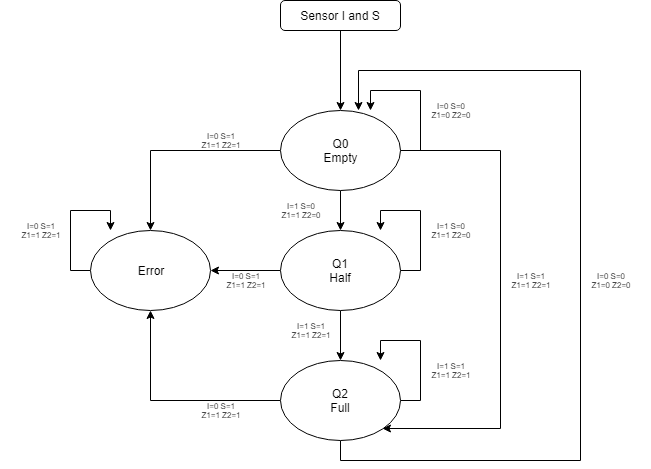
\includegraphics[scale=0.65]{../Exercise1/Mealy/ej1mealy.png}
        \caption{\color{cyan}Exercise 1: Mealy sate machine flow chart}
        \label{fig:ej1mealyd}
    \end{figure}

Which is represented as follow:

% Please add the following required packages to your document preamble:
% \usepackage{multirow}
\begin{table}[H]
\centering
\begin{tabular}{|c|c|c|c|c|c|c|c|c|c|c|}
\hline
\multicolumn{3}{|c|}{\multirow{2}{*}{\textbf{State(Q)}}} & \multicolumn{8}{c|}{\textbf{Input(X)}} \\ \cline{4-11} 
\multicolumn{3}{|c|}{} & \multicolumn{2}{c|}{\textbf{I=0 S=0}} & \multicolumn{2}{c|}{\textbf{I=0 S=1}} & \multicolumn{2}{c|}{\textbf{I=1 S=0}} & \multicolumn{2}{c|}{\textbf{I=1 S=1}} \\ \hline
\textbf{Representation} & \textbf{Q2} & \textbf{Q1} & \textbf{Q2} & \textbf{Q1} & \textbf{Q2} & \textbf{Q1} & \textbf{Q2} & \textbf{Q1} & \textbf{Q2} & \textbf{Q1} \\ \hline
\textbf{Empty} & 0 & 0 & 0 & 0 & 0 & 1 & 1 & 0 & 1 & 1 \\ \hline
\textbf{Error} & 0 & 1 & 0 & 0 & 0 & 1 & 1 & 0 & 1 & 1 \\ \hline
\textbf{Half} & 1 & 0 & 0 & 0 & 0 & 1 & 1 & 0 & 1 & 1 \\ \hline
\textbf{Full} & 1 & 1 & 0 & 0 & 0 & 1 & 1 & 0 & 1 & 1 \\ \hline
\textbf{Output(Z)} & \textbf{Z1} & \textbf{Z2} & \textbf{0} & \textbf{0} & \textbf{1} & \textbf{1} & \textbf{1} & \textbf{0} & \textbf{1} & \textbf{1} \\ \hline
\end{tabular}
\caption{\color{cyan}Exercise 1: Mealy sate machine}
\end{table}

%\pagebreak
So the logic circuit would be:

 \begin{figure}[H]
        \centering
        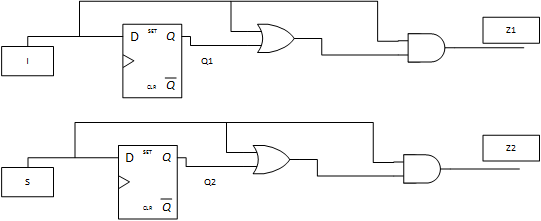
\includegraphics[scale=1]{../Exercise1/Mealy/ej1mealycircuit.png}
        \caption{\color{cyan}Exercise 1: Mealy logic circuit}
        \label{fig:ej1mealyld}
    \end{figure}

We can notice that the input event and the output event are the same which could make the $Z_N=X_N$ with N: the output or input number, but as mention be in the Mealy state machine the output $Z=f(X_1.....X_n,Q_1....Q_n)$, so we considered essential the use of sate in the circuit is dependent with the state and the input to have a clear view of being a Mealy state machine.

\subsubsection{\color{Orange}Simulation}

For the simulation of this stage machine, as the pump B1 and B2 alternate their function when $I = 1 y S = 0$ and for the activation of the pump that depends on output voltage is needed the following circuit is added:

 \begin{figure}[H]
        \centering
        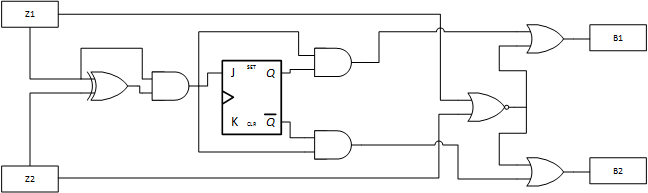
\includegraphics[scale=1]{../Exercise1/Mealy/ej1mealycircuitplus.png}
        \caption{\color{cyan}Exercise 1: Mealy additional logic circuit for the simulation}
        \label{fig:ej1mealylp}
    \end{figure}
    
Simulation the complete circuit in Verilog and testing the possibles values of input in Gtkwave the result was:

 \begin{figure}[H]
        \centering
        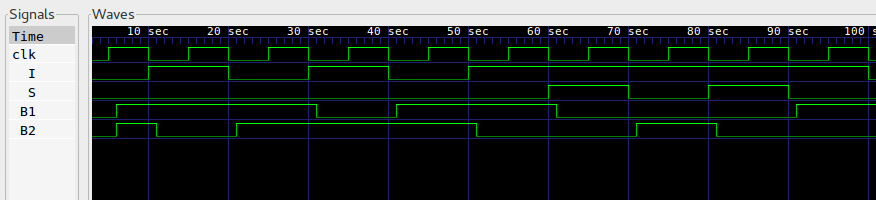
\includegraphics[scale=0.7]{../Exercise1/Mealy/ej1mealysim1.png}\\
        \vspace{0.2cm}
        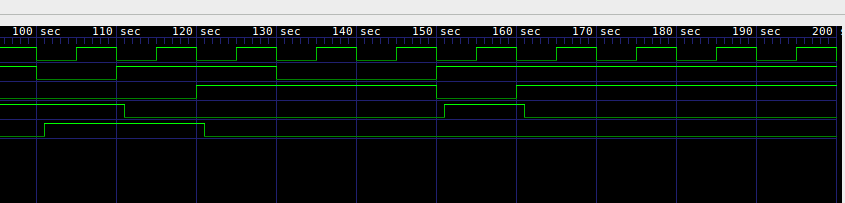
\includegraphics[scale=0.73]{../Exercise1/Mealy/ej1mealysim2.png}
        \caption{\color{cyan}Exercise 1: Simulation results}
        \label{fig:ej1mealyw}
    \end{figure}

%%%%%%%%%%%%%%%%%%%%%%%%%%%%%%%%%%%%%%%%

  

%%%%%%%%%%%%%%%%%%%%%%%%%%%%%%%%%%%%%%%


%\end{document}